\documentclass[12pts]{article}
\usepackage{xcolor, colortbl}
\usepackage{algorithm}
\usepackage[noend]{algpseudocode}
\usepackage{textcomp}
\usepackage{listings}
\usepackage{hyperref}
\usepackage{alltt}
\usepackage{tikz}
\usepackage{framed}
\usepackage{mdframed}
\usepackage{marvosym}
\usepackage{amssymb}
\usepackage{wasysym}
\usepackage{marvosym}
\usepackage{crayola}
\usepackage{mathpartir}
\usepackage{tabularx}
\usepackage[belowskip=-15pt,aboveskip=0pt]{caption}
\usepackage[skins]{tcolorbox}
\usepackage{multicol}
\usetikzlibrary{positioning,shapes,arrows, backgrounds, fit, shadows}
\usetikzlibrary{arrows.meta}
\usetikzlibrary{decorations.markings}
\usepackage[margin=1in]{geometry}

\title{SE Lab Website -- Maintenance Manual}
\author{Sujit Kumar Chakrabarti}

\begin{document}
\maketitle

\section{Object Model}
\begin{center}
\resizebox{\textwidth}{!}{
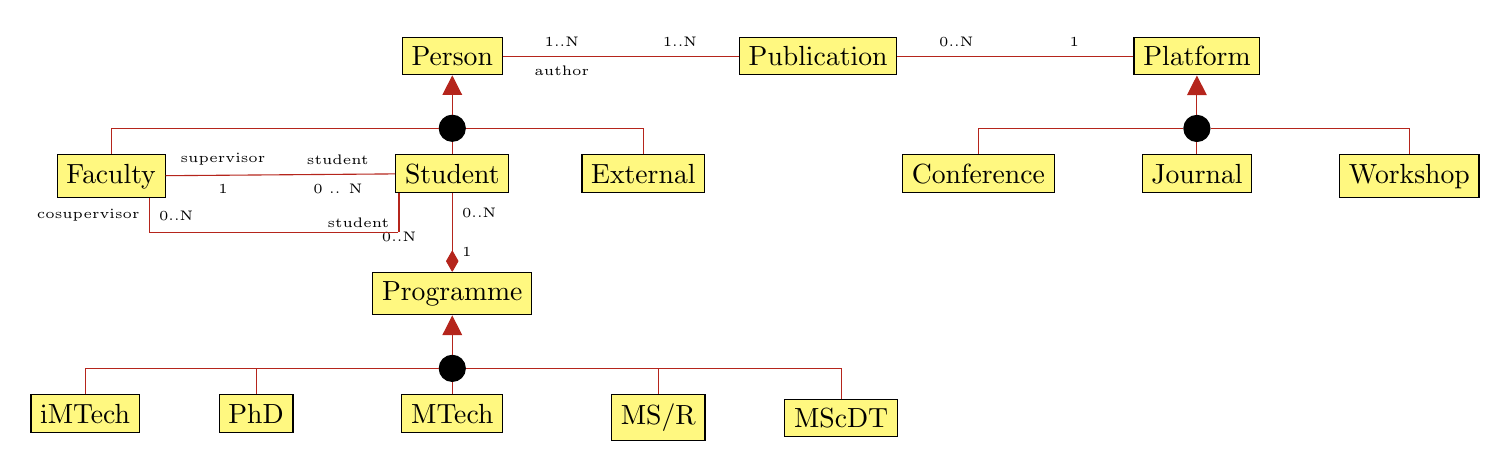
\begin{tikzpicture}
\node[rectangle, draw=black, fill=yellow!50](person) {Person};
\node[rectangle, draw=black, fill=yellow!50, below left=of person, xshift=-2cm](faculty) {Faculty};
\node[rectangle, draw=black, fill=yellow!50, below right=of person](external) {External};
\node[rectangle, draw=black, fill=yellow!50, below= of person](student) {Student};

\node[circle, draw=black, fill=black, minimum height=0, minimum width=0, below=0.5cm of person](j1) {}; 

\draw[BrickRed, arrows={-Triangle[length=0.25cm, width=0.25cm]}] (j1) to (person);
\draw[BrickRed, -] (faculty) |- (j1);
\draw[BrickRed, -] (external) |- (j1);
\draw[BrickRed, -] (student) to (j1);

\draw[-, BrickRed](student) -- 
	node[black, near start, above]{\tiny{student}}
	node[black, near start, below]{\tiny{0 .. N}}
	node[black, near end, above]{\tiny{supervisor}}
	node[black, near end, below]{\tiny{1}}
	(faculty); 
	
\node[circle, draw=black, fill=black, minimum height=0, minimum width=0, inner sep=0, below=0.5cm of student.200](j4) {};

\draw [-, BrickRed] (student.200) -- 
	node[black, near end, left]{\tiny{student}}
	node[black, near end, below]{\tiny{0..N}}
	(j4); 
\draw [-, BrickRed] (j4) -|
	node[black, near end, left]{\tiny{cosupervisor}}
	node[black, near end, right]{\tiny{0..N}}
		(faculty.-30); 


\node[rectangle, draw=black, fill=yellow!50, right= 3cm of person](publication) {Publication};

\node[rectangle, draw=black, fill=yellow!50, right = 3cm of publication](platform) {Platform};
\node[rectangle, draw=black, fill=yellow!50, below left=of platform](conference) {Conference};
\node[rectangle, draw=black, fill=yellow!50, below right=of platform](workshop) {Workshop};
\node[rectangle, draw=black, fill=yellow!50, below= of platform](journal) {Journal};

\node[circle, draw=black, fill=black, minimum height=0, minimum width=0, below=0.5cm of platform](j2) {}; 

\draw[BrickRed, arrows={-Triangle[length=0.25cm, width=0.25cm]}] (j2) to (platform);
\draw[BrickRed, -] (conference) |- (j2);
\draw[BrickRed, -] (workshop) |- (j2);
\draw[BrickRed, -] (journal) to (j2);

\node[rectangle, draw=black, fill=yellow!50, below = of student](programme) {Programme};
\node[rectangle, draw=black, fill=yellow!50, below left=of programme](phd) {PhD};
\node[rectangle, draw=black, fill=yellow!50, left=of phd](imtech) {iMTech};
\node[rectangle, draw=black, fill=yellow!50, below right=of programme](msr) {MS/R};
\node[rectangle, draw=black, fill=yellow!50, below= of programme](mtech) {MTech};
\node[rectangle, draw=black, fill=yellow!50, right=of msr](mscdt) {MScDT};
\node[circle, draw=black, fill=black, minimum height=0, minimum width=0, below=0.5cm of programme](j3) {}; 

\draw[BrickRed, arrows={-Triangle[length=0.25cm, width=0.25cm]}] (j3) to (programme);
\draw[BrickRed, -] (phd) |- (j3);
\draw[BrickRed, -] (msr) |- (j3);
\draw[BrickRed, -] (mtech) to (j3);
\draw[BrickRed, -] (imtech) |- (j3);
\draw[BrickRed, -] (mscdt) |- (j3);

\draw[BrickRed, -] (person) to 
	node[black, above, near start]{\tiny{1..N}}
	node[black, below, near start]{\tiny{author}}
	node[black, above, near end]{\tiny{1..N}}
	(publication);

\draw[BrickRed, -] (publication) to 
	node[black, above, near start]{\tiny{0..N}}
	node[black, above, near end]{\tiny{1}}
	(platform);
	
\draw[BrickRed, -diamond](student) to
	node[black, right, near start]{\tiny{0..N}}
	node[black, right, near end]{\tiny{1}}
 (programme);

\end{tikzpicture}
}
\end{center}

\end{document}